\documentclass{article}
\usepackage{natbib}
\usepackage{graphicx}
%\\bibliographystyle{abbrvnat}
\begin{document}
In SCHISM, the bottom drag coefficient is calculated with the roughness height \citep{Zhang08} as below :

\begin{equation}
C_D = \left( \frac{1}{\kappa_0} \ln \frac{\delta_b}{z_0}\right) ^ {-2}
\end{equation}
where $\kappa_0$ is the von Karman's constant, $z_0$  the bottom roughness, and $\delta_b$ the thickness of the bottom computational cell.
This equation is the drag formula as discussed in \citet{Blumberg87p1}.

But $C_D$ tends to become large when $\delta_b$ is small, which can happen in a shallow area within the $s$-grid system and possibly cause instability. To prevent this, we proposed a limit of $C_D$ as follows:
\begin{equation}
C_D = \left( \frac{1}{\kappa_0} \ln \frac{\tilde \delta_b}{z_0}\right) ^ {-2}
\end{equation}
where $\tilde \delta_b = \max (\delta_b, \delta_{b_{\min}})$ or an attenuation of the $C_D$ by multiplying with an exponential function:
\begin{equation}
C_D = \left( \frac{1}{\kappa_0} \ln \frac{\tilde \delta_b}{z_0}\right) ^ {-2} e ^ {-\lambda ( 1- \delta_b / \tilde \delta_b) }
\end{equation}
where $\lambda$ is a decay coefficient. The proposed $C_D$ is plotted in the figure below.

\begin{figure}
\centering
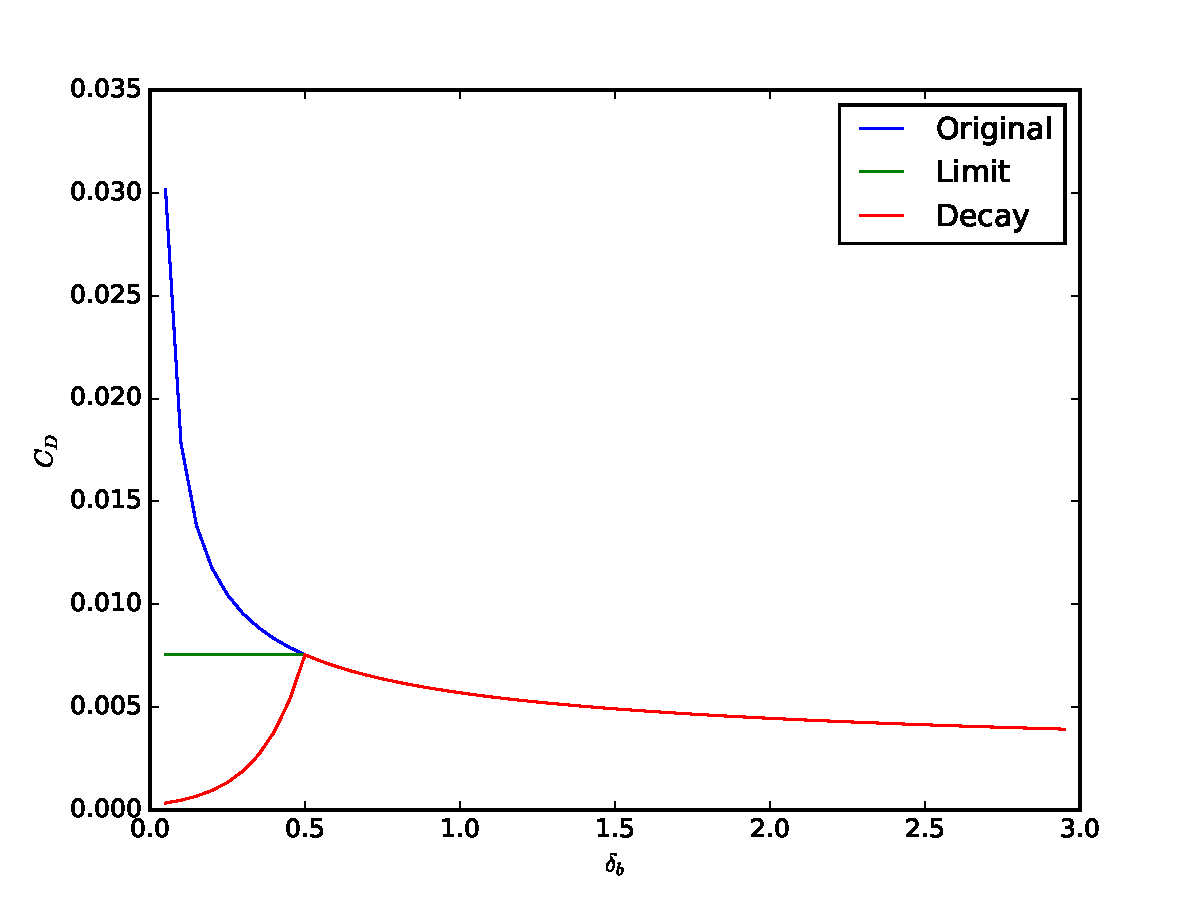
\includegraphics[width=\textwidth]{image/cd}
\caption{$C_D$ values by three different methods of calculation, $z_0$ = 0.005, $\delta_{b_{\max}}=0.5$, $\lambda=3.459$}
\end{figure}

%\bibliography{references}
 \end{document}
